\subsubsection{Contenido de la sección ``Detalles de la campaña''}
El contenido de la sección está dividido en 8 Cards diferentes.

La primera Card es la de ``Mis puntos'', el usuario puede ver un historial de las solicitudes de puntos que ha realizado. Si el usuario nunca ha realizado una solicitud de puntos, en la Card sólo le mostrará un mensaje indicándole esto (Ver Figura 12).

    \begin{figure}[H]
        \begin{center}
            
\includegraphics[scale=0.60]{img/actividades/detalles-campanias/card-puntos.png}
            \caption{Card de puntos sin contenido.}
            \label{fig:card-puntos}
        \end{center}
    \end{figure}

Pero si el usuario ya tiene solicitudes hechas, se le mostrarán máximo las últimas 6 solicitudes que ha realizado con información general de la solicitud como la imagen de la evidencia que se subió, la cantidad de puntos que se solicitaron, la fecha en la que se realizó la solicitud y el estatus de la misma (Ver Figura 13).

    \begin{figure}[H]
        \begin{center}
            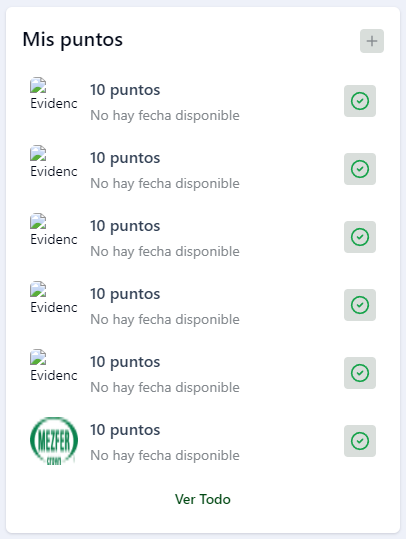
\includegraphics[scale=0.60]{img/actividades/detalles-campanias/card-puntos-contenido.png}
            \caption{Card de puntos con contenido.}
            \label{fig:card-puntos-contenido}
        \end{center}
    \end{figure}

Si el usuario quisiera ver todas las solicitudes que ha realizado, puede presionar el botón que se encuentra en la parte inferior de la Card con la leyenda ``Ver Todo''. Al presionarlo, se mostrará un componente llamado ``Dialog'' y su contenido dependerá de la cantidad de solicitudes hechas; si no hay ninguna, el Dialog sólo contendrá un mensaje indicando esto. (Ver Figura 14).

    \begin{figure}[H]
        \begin{center}
            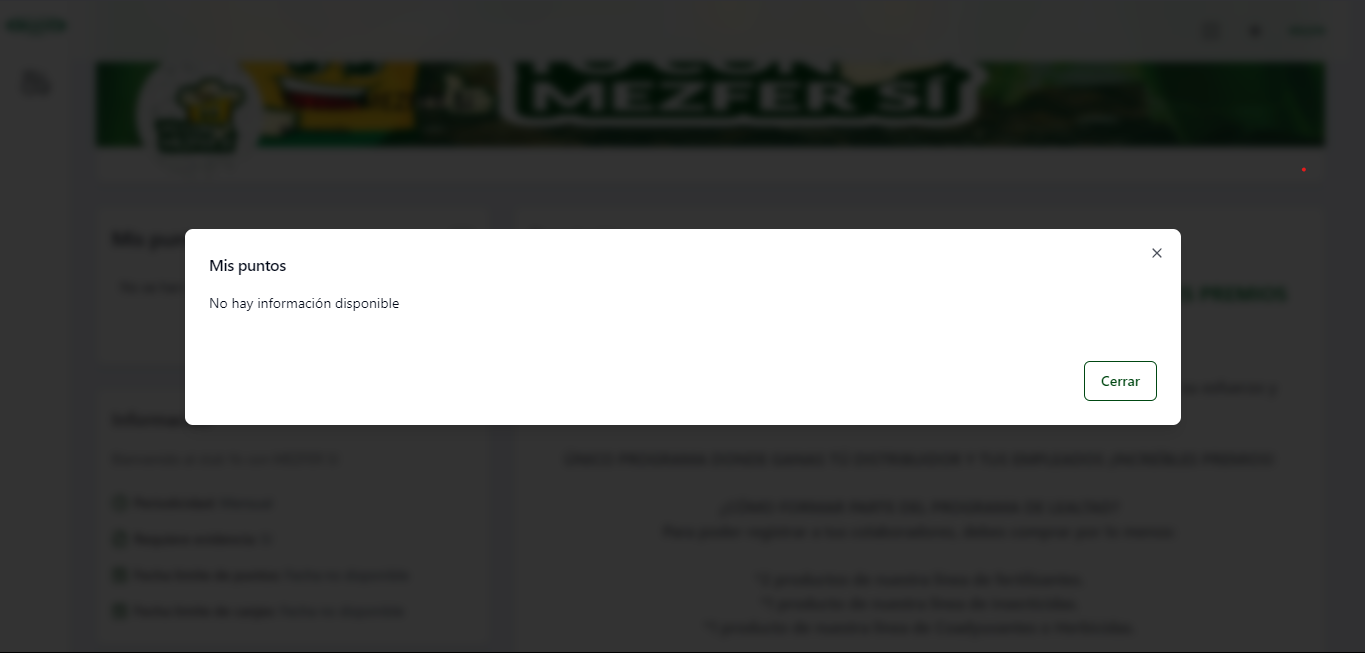
\includegraphics[scale=0.35]{img/actividades/detalles-campanias/dialog-puntos-vacio.png}
            \caption{Dialog de puntos vacío.}
            \label{fig:dialog-puntos-vacio}
        \end{center}
    \end{figure}

Si ya hay solicitudes, el Dialog contendrá una tabla con la información de todas las solicitudes (Ver Figura 15).

    \begin{figure}[H]
        \begin{center}
            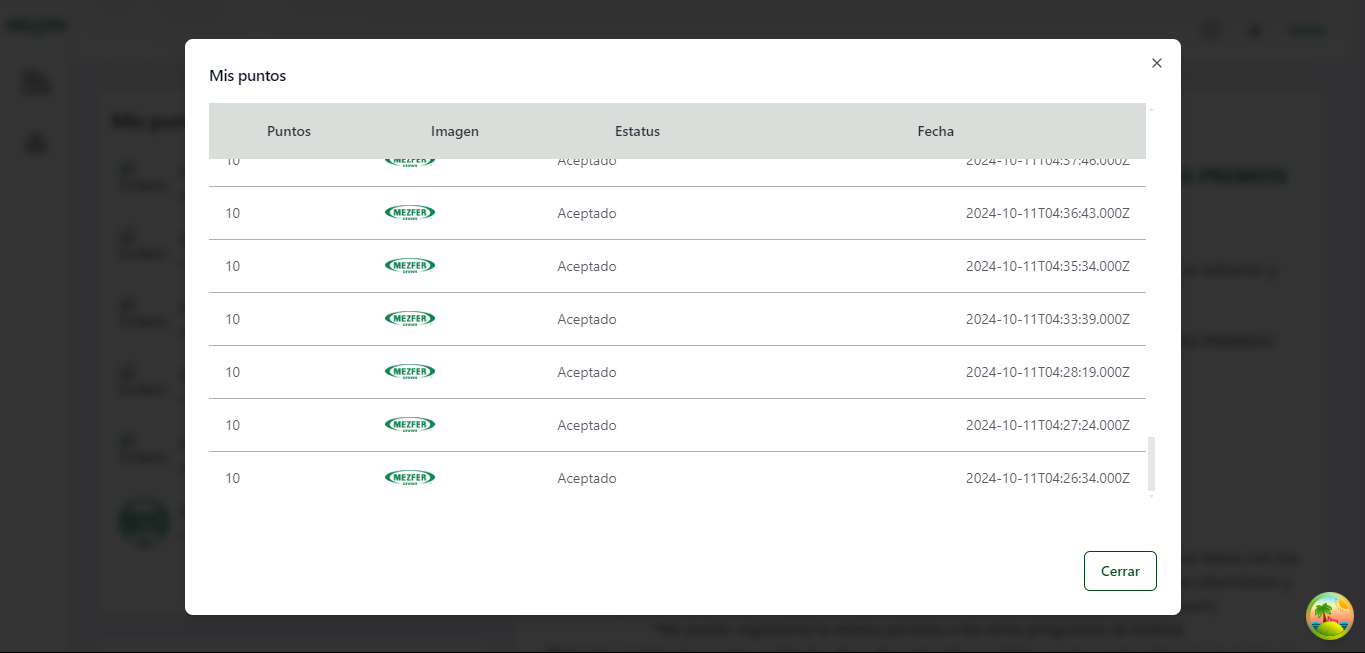
\includegraphics[scale=0.35]{img/actividades/detalles-campanias/dialog-puntos-contenido.png}
            \caption{Dialog de puntos con contenido.}
            \label{fig:dialog-puntos-contenido}
        \end{center}
    \end{figure}

Otra característica importante de esta Card es que permite realizar una solicitud de puntos, esto se hace mediante el botón con un ícono ``+'' que se encuentra en la esquina superior derecha. Al presionarlo, al usuario se le mostrará un Dialog con un formulario para que ingrese toda la información necesaria (Ver Figura 16).

    \begin{figure}[H]
        \begin{center}
            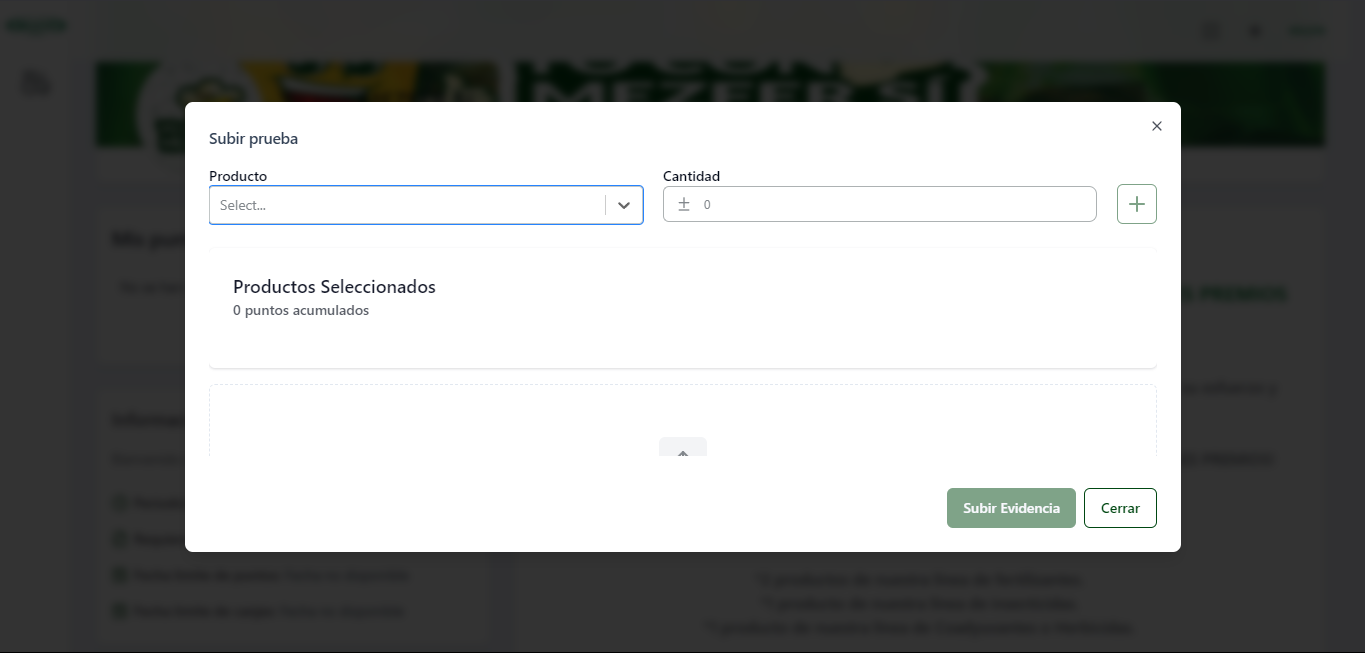
\includegraphics[scale=0.35]{img/actividades/detalles-campanias/dialof-formulario.png}
            \caption{Dialog con formulario para realizar la solicitud.}
            \label{fig:dialog-solicitud}
        \end{center}
    \end{figure}

En la segunda Card se muestra información relevante de la campaña respecto a la periodicidad de esta y las fechas de solicitudes y canjes de los puntos (Ver Figura 17).

    \begin{figure}[H]
        \begin{center}
            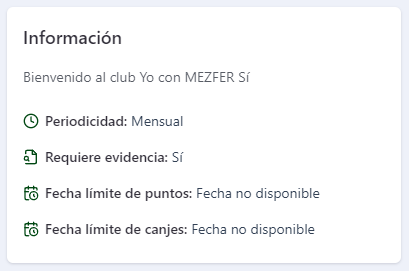
\includegraphics[scale=0.60]{img/actividades/detalles-campanias/card-info-puntos.png}
            \caption{Card con información de la campaña.}
            \label{fig:card-info-campanias}
        \end{center}
    \end{figure}

La tercera Card es donde el usuario puede canjear sus puntos por un premio. Hasta el momento de la redacción de este reporte, esta funcionalidad no está implementada, en la Card sólo se ve un botón pero al presionarlo no ocurre nada (Ver Figura 18).

    \begin{figure}[H]
        \begin{center}
            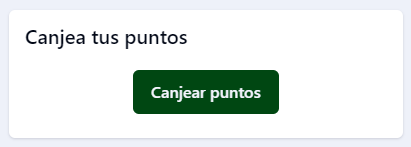
\includegraphics[scale=0.60]{img/actividades/detalles-campanias/card-canje.png}
            \caption{Card de canje de puntos.}
            \label{fig:card-canje}
        \end{center}
    \end{figure}

La cuarta Card muestra los premios que se pueden obtener en la campaña. A simple vista, al usuario se le muestran 6 premios como máximo y sus respectivos detalles como la imagen del premio, el nombre y la cantidad de puntos que se requieren para obtenerlo (Ver Figura 19).

    \begin{figure}[H]
        \begin{center}
            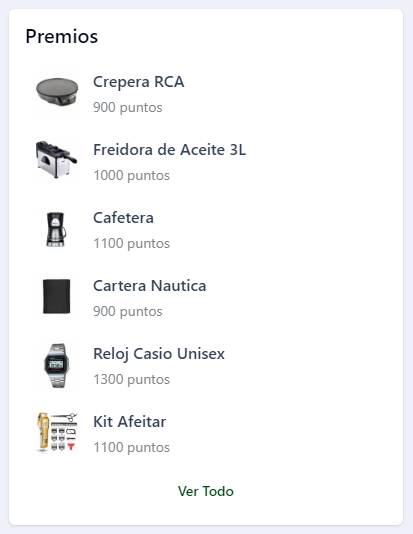
\includegraphics[scale=0.60]{img/actividades/detalles-campanias/card-premios.png}
            \caption{Card con los premios de las campañas.}
            \label{fig:card-premios}
        \end{center}
    \end{figure}

Si el usuario quisiera ver todos los premios disponibles, deberá presionar el botón con la leyenda ``Ver Todo'' que se encuentra en la parte inferior de la Card. Al presionarlo, se mostrará un Dialog con una tabla que contiene la información de todos los premios (Ver Figura 20).

    \begin{figure}[H]
        \begin{center}
            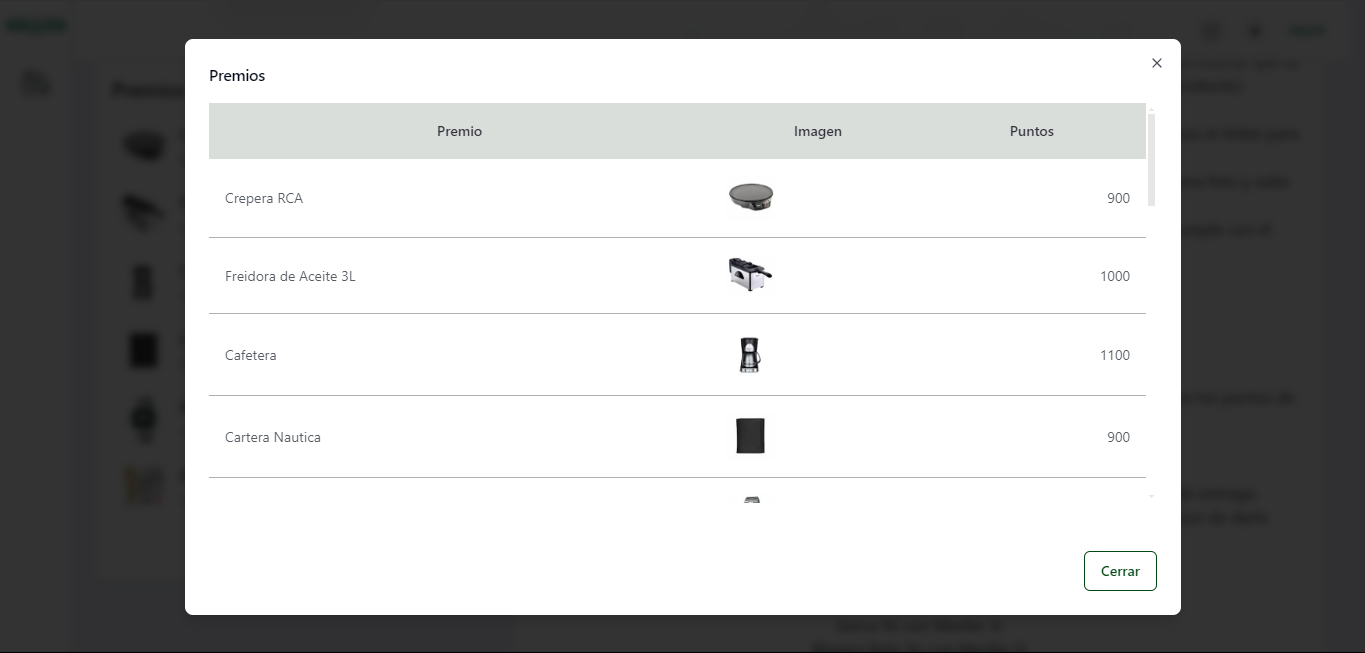
\includegraphics[scale=0.33]{img/actividades/detalles-campanias/dialog-premios.png}
            \caption{Dialog con los premios de la campaña.}
            \label{fig:dialog-premios}
        \end{center}
    \end{figure}

La quinta Card es donde se muestra la descripción de la campaña. En la base de datos, las descripciones están guardadas con información que permite darles el orden y el formato adecuado:
    \begin{itemize}
        \item Número: Este número indica el orden de cada párrafo de la descripción.
        \item Tipo: A cada párrafo se le asigna un tipo como título, subtítulo, información, etc., de esta manera se le puede asignar un color.
    \end{itemize}

Para poder dar un formato aduecuado de todo el texto en la Card, se utilizan arreglos y objetos: en el arreglo se ordenan los párrafos para que el texto tenga sentido, y en el objeto se crean pares llave/valor para que, de acuerdo al tipo de la descripción, se le asigne un color. Otro punto importante es que en la base de datos, el texto de cada párrafo tiene caracteres especiales para indicar los saltos de línea; si este texto se muestra sin darle un formato, estos caracteres también se mostrarán, por lo que es importante que el código pueda identificar estos caracteres y saber que se trata de saltos de línea, y para lograr esto se hace uso de expresiones regulares.

Cubiertos todos estos aspectos, la descripción de la campaña se puede colocar correctamente en la Card (Ver Figura 21).

    \begin{figure}[H]
        \begin{center}
            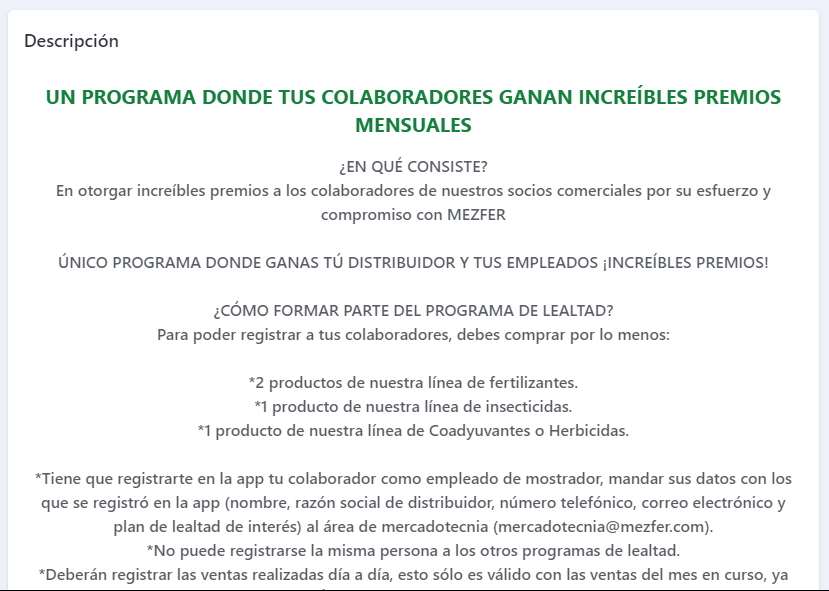
\includegraphics[scale=0.40]{img/actividades/detalles-campanias/card-descripcion.png}
            \caption{Card con la descripcion de la campaña.}
            \label{fig:card-descripcion}
        \end{center}
    \end{figure}

En la sexta Card, se muestra el cuadro de equivalencias de la campaña. Este cuadro de equivalencias muestra todos los productos participantes y la cantidad de puntos que se pueden ganar al comprarlos (Ver Figura 22).

    \begin{figure}[H]
        \begin{center}
            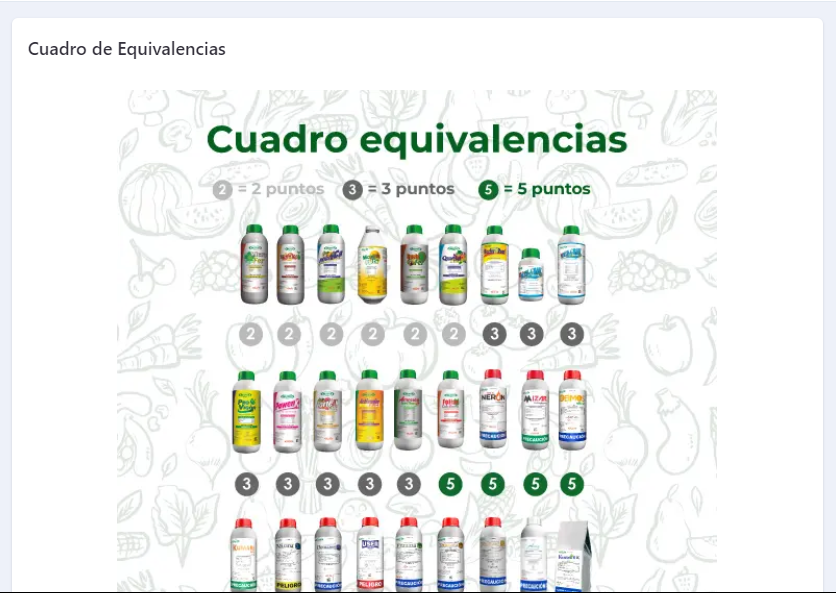
\includegraphics[scale=0.40]{img/actividades/detalles-campanias/card-equivalencias.png}
            \caption{Card con el cuadro de equivalencias.}
            \label{fig:card-equivalencias}
        \end{center}
    \end{figure}

La séptima Card contiene una tabla con los productos que participan en la campaña. Esta tabla está paginada, cada página contiene como máximo 7 productos; también se puede realizar la búsqueda de un producto mediante su nombre con el campo que se encuentra en la parte superior de la tabla, este campo va filtrando el arreglo con todos los productos y retorna las coincidencias que haya con lo que el usuario haya escrito. (Ver Figura 23). 

    \begin{figure}[H]
        \begin{center}
            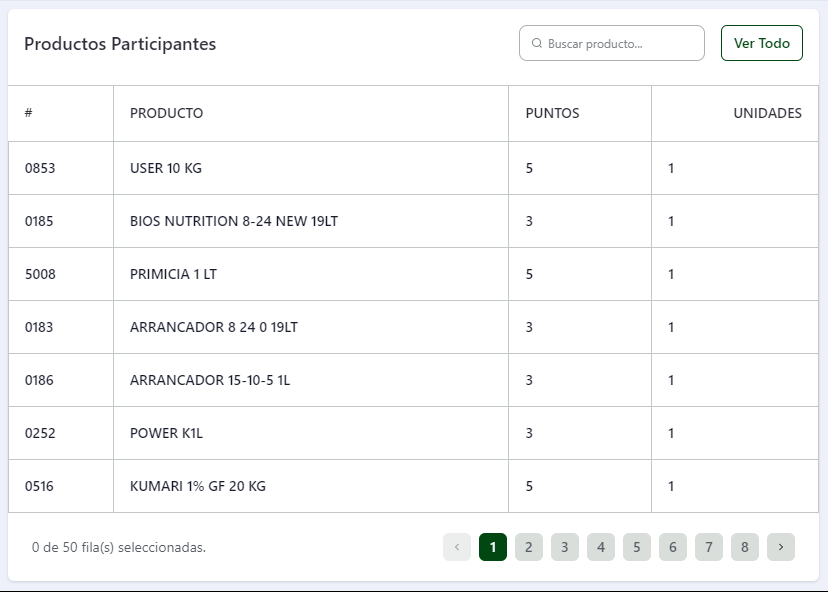
\includegraphics[scale=0.40]{img/actividades/detalles-campanias/card-productos-participantes.png}
            \caption{Card con los productos participantes.}
            \label{fig:card-productos-participantes}
        \end{center}
    \end{figure}

Si el usuario no quisiera navegar por las páginas de la tabla, puede presionar el botón con la leyenda ``Ver Todo'' que se encuentra en la esquina superior derecha. Este botón mostrará un Dialog con una tabla con todos los productos (Ver Figura 24).

    \begin{figure}[H]
        \begin{center}
            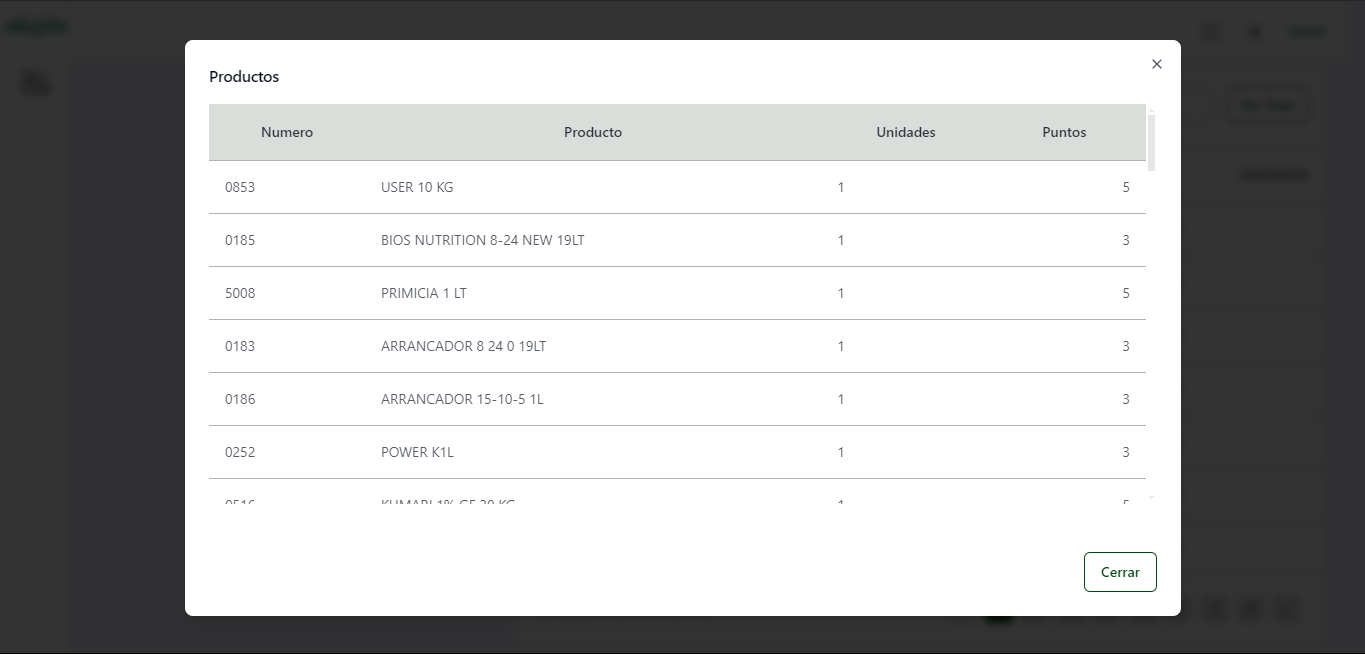
\includegraphics[scale=0.35]{img/actividades/detalles-campanias/dialog-productos-participantes.png}
            \caption{Dialog con los productos de la campaña.}
            \label{fig:dialog-productos-participantes}
        \end{center}
    \end{figure}

La octava y última Card de esta sección contiene una tabla en la que el usuario podrá ver todos los canjes que ha realizado, esta tabla también contiene un campo que permite al usuario buscar cierto canje que haya realizado. Al igual que en Cards anteriores, si el usuario no ha realizado ningún canje, la Card contendrá un mensaje indicándole esto (Ver Figura 25).

    \begin{figure}[H]
        \begin{center}
            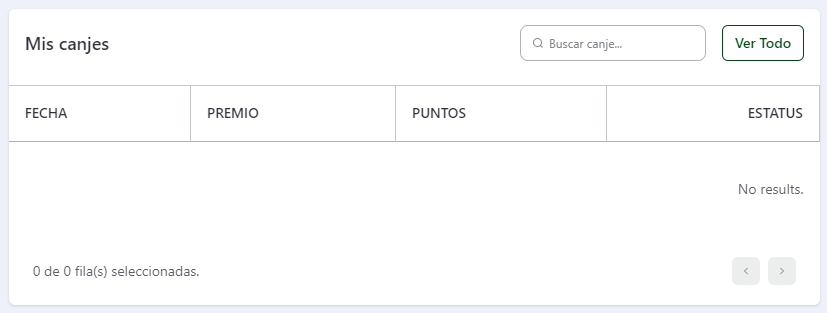
\includegraphics[scale=0.50]{img/actividades/detalles-campanias/card-canjes.png}
            \caption{Card de canjes sin contenido.}
            \label{fig:card-canjes}
        \end{center}
    \end{figure}

Al presionar el botón con la leyenda ``Ver Todo'' que se encuentra en la esquina superior derecha, al usuario se le mostrará un Dialog con una tabla sin paginación con todos los canjes que ha realizado. En este caso, como no hay información que mostrar, sólo se mostrará un mensaje indicando esto (Ver Figura 26).

    \begin{figure}[H]
        \begin{center}
            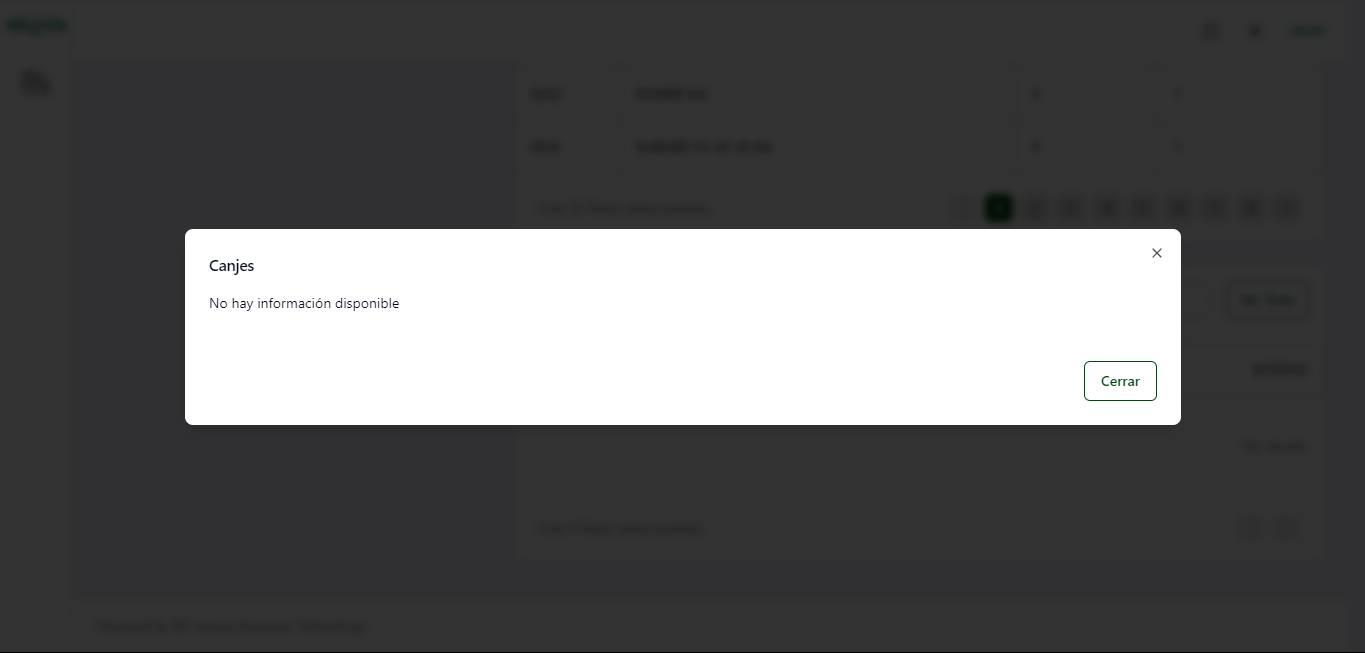
\includegraphics[scale=0.35]{img/actividades/detalles-campanias/dialog-canjes-vacio.png}
            \caption{Dialog de canjes sin contenido.}
            \label{fig:dialog-canjes-vacio}
        \end{center}
    \end{figure}

Si ya hay canjes realizados, el usuario podrá ver todos los detalles de estos (Ver Figura 27).

    \begin{figure}[H]
        \begin{center}
            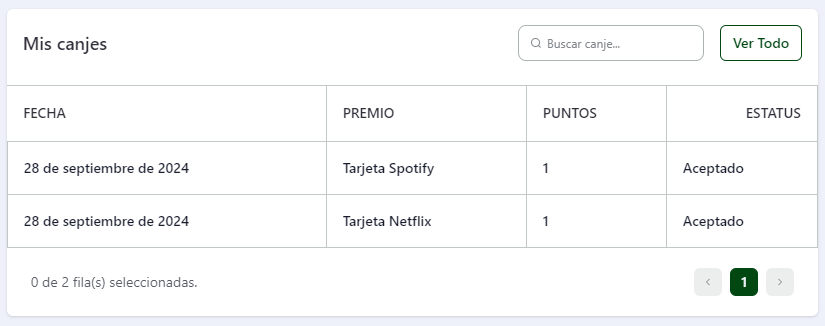
\includegraphics[scale=0.50]{img/actividades/detalles-campanias/card-canjes-contenido.png}
            \caption{Card de canjes con contenido.}
            \label{fig:card-canjes-contenido}
        \end{center}
    \end{figure}

Y esta misma información la podrá ver en el Dialog con una tabla sin paginación que se muestra al presionar el botón ``Ver Todo'' (Ver Figura 28).

\begin{figure}[H]
    \begin{center}
        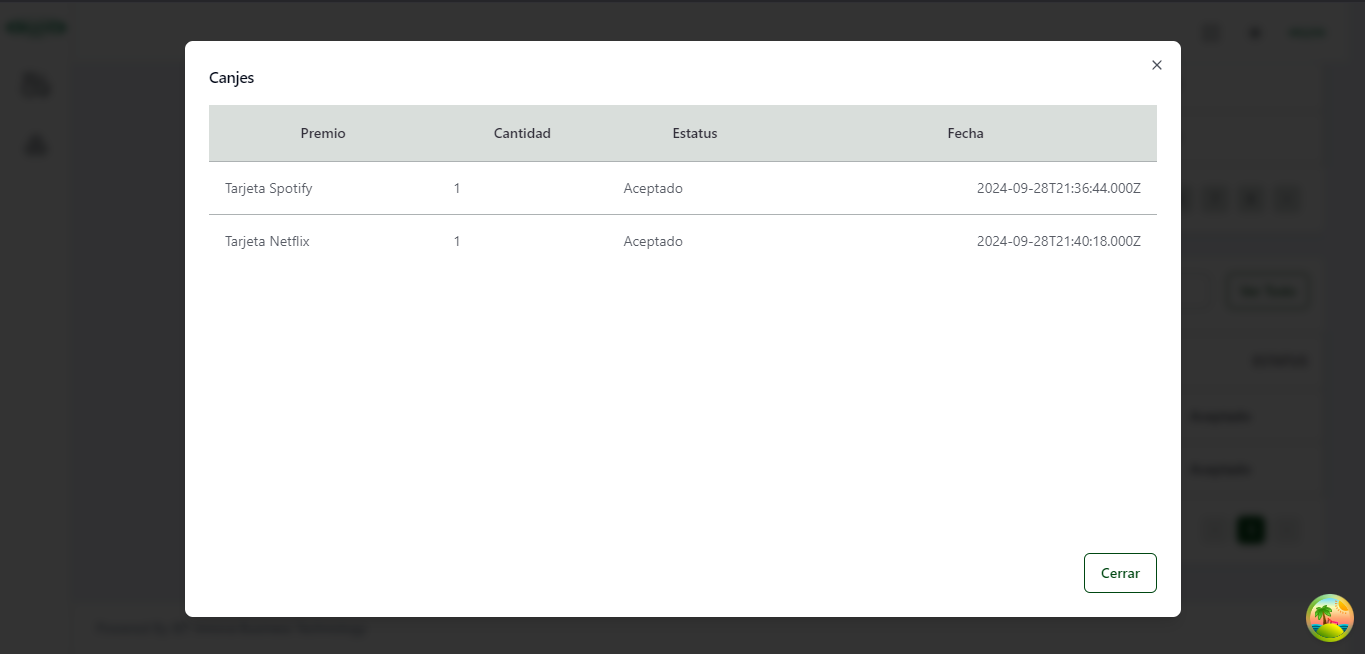
\includegraphics[scale=0.32]{img/actividades/detalles-campanias/dialog-canjes-contenido.png}
        \caption{Dialog de canjes con contenido.}
        \label{fig:dialog-canjes-contenido}
    \end{center}
\end{figure}